\section{Prototipagem}
Segundo \citeonline{ferreira:2020}, ``prototipar é trazer, para o mundo real, o mundo palpável, as ideias de negócio construídas no mundo abstrato, na teoria''. Isto é, o autor comenta que um protótipo é um recurso utilizado para demonstrar e escolher a solução para representar uma ideia, podendo ser efetuado com entregas digitais, como telas de sistema. Dado isto, a próxima seção apresentará as telas prototipadas do projeto de sistema \gls{ifriends}.

Ainda, para auxiliar na prototipação das telas, foi elaborado um mapa mental de modo a representar melhor o fluxo do nosso projeto, que pode ser conferido na \autoref{Mapa mental}.

\begin{figure}[htb]
\centering
\caption{\label{Mapa mental} Mapa mental}
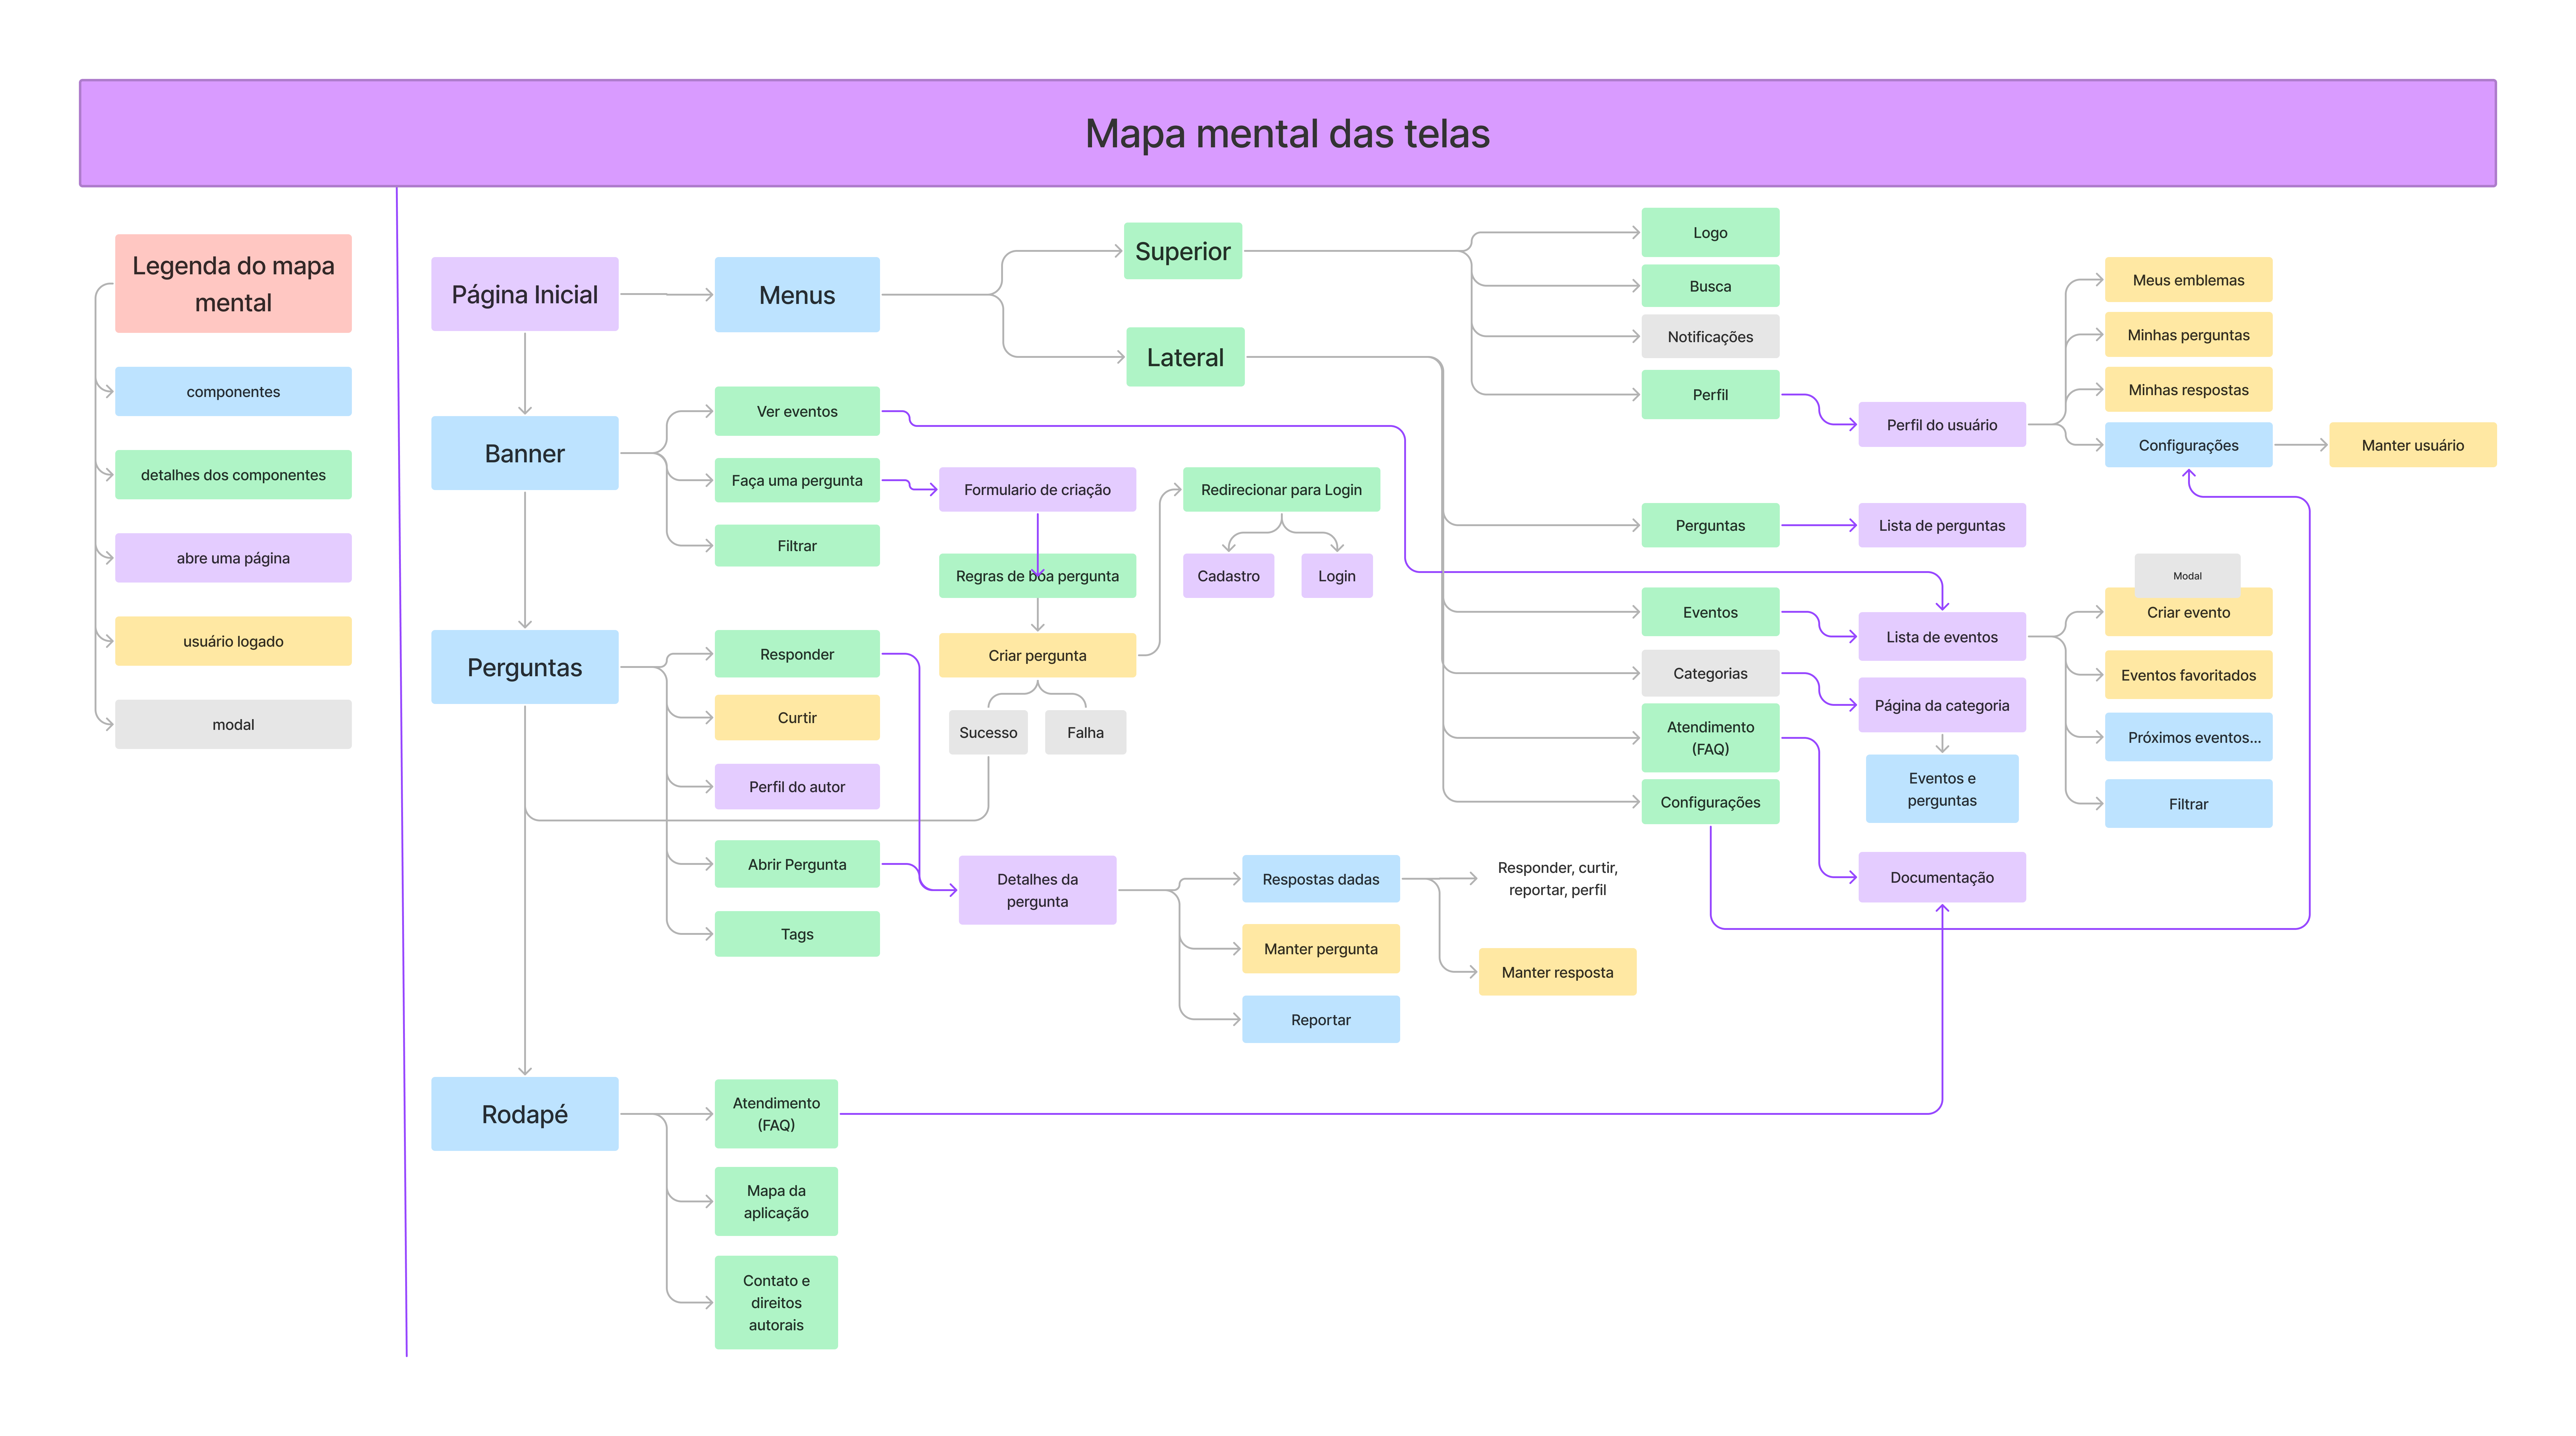
\includegraphics[width=1\textwidth]{anexos/Imagens_Prototipo/Mapa_Mental.png}
\fonte{os autores}
\end{figure}
\FloatBarrier

\subsection{Protótipos de alta fidelidade}
Nesta seção estão contidas as figuras que representam as principais telas do sistema em relação a \gls{POC} do projeto, cada tela apresenta uma breve contextualização sobre o seu conteúdo. De todo modo, a apresentação pode ser visualizada também pelo \href{https://www.figma.com/proto/GhIlybDubGmr3NkRU0a9GP/Protótipo---IFriends?node-id=73\%3A321}{Figma}.

A \autoref{Home Page} apresenta a página inicial do projeto, onde o usuário entra em contato pela primeira vez com o sistema. Nela o usuário pode navegar através de dois menus disponíveis na página: o lateral e o superior, usar a barra de pesquisa, \textit{logar} no seu perfil, acessar as suas configurações, entre outras ações disponibilizadas. Na página encontram as questões mais relevantes da comunidade, assim como os espaços destinados para a realização de uma pergunta ou de uma monitoria.

\begin{figure}[htb]
\centering
\caption{\label{Home Page} Página inicial}
\includesvg[inkscapelatex=false,width=0.7\textwidth]{anexos/Imagens_Prototipo/Home_Page.svg}
\fonte{os autores}
\end{figure}
\FloatBarrier

Quando o usuário clica em uma pergunta ou em ``Responder'' ele é direcionado à página dessa pergunta como mostra a \autoref{Pergunta e respostas}, nela ele pode encontrar as respostas já fornecidas por outros membros da comunidade, assim como também pode deixar a sua contribuição.

\begin{figure}[htb]
\centering
\caption{\label{Pergunta e respostas} Pergunta e respostas}
\includesvg[inkscapelatex=false,width=0.9\textwidth]{anexos/Imagens_Prototipo/Pergunta_Respostas.svg}
\fonte{os autores}
\end{figure}
\FloatBarrier

Já a \autoref{Cadastro de perguntas} corresponde a página de cadastro de perguntas, nessa tela são apresentados todos os elementos julgados necessários para a sua realização, nesta página ainda de encontra o manual de uma boa pergunta, tal foi elaborado com o intuito de ajudar e auxiliar o usuário na preparação de sua problemática. 

\begin{figure}[htb]
\centering
\caption{\label{Cadastro de perguntas} Cadastro de perguntas}
\includesvg[inkscapelatex=false,width=0.9\textwidth]{anexos/Imagens_Prototipo/Cadastro_Perguntas.svg}
\fonte{os autores}
\end{figure}
\FloatBarrier

As telas apresentadas até o momento são aquelas que se encontram relacionadas com a \gls{POC}, portanto vale salientar que esta seção será atualizada futuramente conforme o andamento e elaboração do projeto.
